% Options for packages loaded elsewhere
\PassOptionsToPackage{unicode}{hyperref}
\PassOptionsToPackage{hyphens}{url}
%
\documentclass[
]{article}
\usepackage{amsmath,amssymb}
\usepackage{iftex}
\ifPDFTeX
  \usepackage[T1]{fontenc}
  \usepackage[utf8]{inputenc}
  \usepackage{textcomp} % provide euro and other symbols
\else % if luatex or xetex
  \usepackage{unicode-math} % this also loads fontspec
  \defaultfontfeatures{Scale=MatchLowercase}
  \defaultfontfeatures[\rmfamily]{Ligatures=TeX,Scale=1}
\fi
\usepackage{lmodern}
\ifPDFTeX\else
  % xetex/luatex font selection
\fi
% Use upquote if available, for straight quotes in verbatim environments
\IfFileExists{upquote.sty}{\usepackage{upquote}}{}
\IfFileExists{microtype.sty}{% use microtype if available
  \usepackage[]{microtype}
  \UseMicrotypeSet[protrusion]{basicmath} % disable protrusion for tt fonts
}{}
\makeatletter
\@ifundefined{KOMAClassName}{% if non-KOMA class
  \IfFileExists{parskip.sty}{%
    \usepackage{parskip}
  }{% else
    \setlength{\parindent}{0pt}
    \setlength{\parskip}{6pt plus 2pt minus 1pt}}
}{% if KOMA class
  \KOMAoptions{parskip=half}}
\makeatother
\usepackage{xcolor}
\usepackage[margin=1in]{geometry}
\usepackage{color}
\usepackage{fancyvrb}
\newcommand{\VerbBar}{|}
\newcommand{\VERB}{\Verb[commandchars=\\\{\}]}
\DefineVerbatimEnvironment{Highlighting}{Verbatim}{commandchars=\\\{\}}
% Add ',fontsize=\small' for more characters per line
\usepackage{framed}
\definecolor{shadecolor}{RGB}{248,248,248}
\newenvironment{Shaded}{\begin{snugshade}}{\end{snugshade}}
\newcommand{\AlertTok}[1]{\textcolor[rgb]{0.94,0.16,0.16}{#1}}
\newcommand{\AnnotationTok}[1]{\textcolor[rgb]{0.56,0.35,0.01}{\textbf{\textit{#1}}}}
\newcommand{\AttributeTok}[1]{\textcolor[rgb]{0.13,0.29,0.53}{#1}}
\newcommand{\BaseNTok}[1]{\textcolor[rgb]{0.00,0.00,0.81}{#1}}
\newcommand{\BuiltInTok}[1]{#1}
\newcommand{\CharTok}[1]{\textcolor[rgb]{0.31,0.60,0.02}{#1}}
\newcommand{\CommentTok}[1]{\textcolor[rgb]{0.56,0.35,0.01}{\textit{#1}}}
\newcommand{\CommentVarTok}[1]{\textcolor[rgb]{0.56,0.35,0.01}{\textbf{\textit{#1}}}}
\newcommand{\ConstantTok}[1]{\textcolor[rgb]{0.56,0.35,0.01}{#1}}
\newcommand{\ControlFlowTok}[1]{\textcolor[rgb]{0.13,0.29,0.53}{\textbf{#1}}}
\newcommand{\DataTypeTok}[1]{\textcolor[rgb]{0.13,0.29,0.53}{#1}}
\newcommand{\DecValTok}[1]{\textcolor[rgb]{0.00,0.00,0.81}{#1}}
\newcommand{\DocumentationTok}[1]{\textcolor[rgb]{0.56,0.35,0.01}{\textbf{\textit{#1}}}}
\newcommand{\ErrorTok}[1]{\textcolor[rgb]{0.64,0.00,0.00}{\textbf{#1}}}
\newcommand{\ExtensionTok}[1]{#1}
\newcommand{\FloatTok}[1]{\textcolor[rgb]{0.00,0.00,0.81}{#1}}
\newcommand{\FunctionTok}[1]{\textcolor[rgb]{0.13,0.29,0.53}{\textbf{#1}}}
\newcommand{\ImportTok}[1]{#1}
\newcommand{\InformationTok}[1]{\textcolor[rgb]{0.56,0.35,0.01}{\textbf{\textit{#1}}}}
\newcommand{\KeywordTok}[1]{\textcolor[rgb]{0.13,0.29,0.53}{\textbf{#1}}}
\newcommand{\NormalTok}[1]{#1}
\newcommand{\OperatorTok}[1]{\textcolor[rgb]{0.81,0.36,0.00}{\textbf{#1}}}
\newcommand{\OtherTok}[1]{\textcolor[rgb]{0.56,0.35,0.01}{#1}}
\newcommand{\PreprocessorTok}[1]{\textcolor[rgb]{0.56,0.35,0.01}{\textit{#1}}}
\newcommand{\RegionMarkerTok}[1]{#1}
\newcommand{\SpecialCharTok}[1]{\textcolor[rgb]{0.81,0.36,0.00}{\textbf{#1}}}
\newcommand{\SpecialStringTok}[1]{\textcolor[rgb]{0.31,0.60,0.02}{#1}}
\newcommand{\StringTok}[1]{\textcolor[rgb]{0.31,0.60,0.02}{#1}}
\newcommand{\VariableTok}[1]{\textcolor[rgb]{0.00,0.00,0.00}{#1}}
\newcommand{\VerbatimStringTok}[1]{\textcolor[rgb]{0.31,0.60,0.02}{#1}}
\newcommand{\WarningTok}[1]{\textcolor[rgb]{0.56,0.35,0.01}{\textbf{\textit{#1}}}}
\usepackage{graphicx}
\makeatletter
\def\maxwidth{\ifdim\Gin@nat@width>\linewidth\linewidth\else\Gin@nat@width\fi}
\def\maxheight{\ifdim\Gin@nat@height>\textheight\textheight\else\Gin@nat@height\fi}
\makeatother
% Scale images if necessary, so that they will not overflow the page
% margins by default, and it is still possible to overwrite the defaults
% using explicit options in \includegraphics[width, height, ...]{}
\setkeys{Gin}{width=\maxwidth,height=\maxheight,keepaspectratio}
% Set default figure placement to htbp
\makeatletter
\def\fps@figure{htbp}
\makeatother
\usepackage{soul}
\setlength{\emergencystretch}{3em} % prevent overfull lines
\providecommand{\tightlist}{%
  \setlength{\itemsep}{0pt}\setlength{\parskip}{0pt}}
\setcounter{secnumdepth}{-\maxdimen} % remove section numbering
\ifLuaTeX
  \usepackage{selnolig}  % disable illegal ligatures
\fi
\IfFileExists{bookmark.sty}{\usepackage{bookmark}}{\usepackage{hyperref}}
\IfFileExists{xurl.sty}{\usepackage{xurl}}{} % add URL line breaks if available
\urlstyle{same}
\hypersetup{
  pdftitle={Part 2. 데이터 전처리},
  hidelinks,
  pdfcreator={LaTeX via pandoc}}

\title{Part 2. 데이터 전처리}
\author{}
\date{\vspace{-2.5em}}

\begin{document}
\maketitle

\hypertarget{uxb370uxc774uxd130-uxbcc0uxd658}{%
\subsubsection{2. 데이터 변환}\label{uxb370uxc774uxd130-uxbcc0uxd658}}

\hypertarget{uxbcc0uxc218}{%
\paragraph{1. 변수}\label{uxbcc0uxc218}}

\begin{quote}
df\$변수명 : 새 변수 생성
\end{quote}

\begin{quote}
transform(df, 변수명=함수) : 새 변수 or 더미 변수 생성
\end{quote}

※ 더미 변수 생성 시, 기준이 되는 범주를 제외한 \ul{(n-1)개의 더미 변수}
생성

\begin{Shaded}
\begin{Highlighting}[]
\FunctionTok{data}\NormalTok{(iris)}
\NormalTok{dt }\OtherTok{\textless{}{-}}\NormalTok{ iris}

\CommentTok{\# df$}
\NormalTok{dt}\SpecialCharTok{$}\NormalTok{Sum.Length }\OtherTok{\textless{}{-}}\NormalTok{ dt}\SpecialCharTok{$}\NormalTok{Sepal.Length}\SpecialCharTok{+}\NormalTok{dt}\SpecialCharTok{$}\NormalTok{Petal.Length}

\CommentTok{\# transform}
\NormalTok{dt\_new }\OtherTok{\textless{}{-}} \FunctionTok{transform}\NormalTok{(dt,}
                    \AttributeTok{Species\_setosa =} \FunctionTok{ifelse}\NormalTok{(Species}\SpecialCharTok{==}\StringTok{\textquotesingle{}setosa\textquotesingle{}}\NormalTok{,}\DecValTok{1}\NormalTok{,}\DecValTok{0}\NormalTok{),}
                    \AttributeTok{Species\_versicolor =} \FunctionTok{ifelse}\NormalTok{(Species}\SpecialCharTok{==}\StringTok{\textquotesingle{}versicolor\textquotesingle{}}\NormalTok{,}\DecValTok{1}\NormalTok{,}\DecValTok{0}\NormalTok{))}
\FunctionTok{head}\NormalTok{(dt\_new)}
\end{Highlighting}
\end{Shaded}

\begin{verbatim}
##   Sepal.Length Sepal.Width Petal.Length Petal.Width Species Sum.Length
## 1          5.1         3.5          1.4         0.2  setosa        6.5
## 2          4.9         3.0          1.4         0.2  setosa        6.3
## 3          4.7         3.2          1.3         0.2  setosa        6.0
## 4          4.6         3.1          1.5         0.2  setosa        6.1
## 5          5.0         3.6          1.4         0.2  setosa        6.4
## 6          5.4         3.9          1.7         0.4  setosa        7.1
##   Species_setosa Species_versicolor
## 1              1                  0
## 2              1                  0
## 3              1                  0
## 4              1                  0
## 5              1                  0
## 6              1                  0
\end{verbatim}

\hypertarget{uxbcc0uxc218-uxcd95uxc18c}{%
\paragraph{2. 변수 축소}\label{uxbcc0uxc218-uxcd95uxc18c}}

\begin{itemize}
\tightlist
\item
  주성분 분석
\end{itemize}

\begin{quote}
princomp(data, cor=FALSE, scores=TRUE) : 주성분분석

\begin{itemize}
\item
  cor : TRUE=상관행렬로(측정단위 표준화) /FALSE=공분산행렬로(측정단위
  반영)
\item
  scores : 각 주성분의 점수를 계산해야 하는지 =\textgreater{} 주성분들의
  선형식을 통해 각 행별 좌표 계산
\end{itemize}
\end{quote}

\begin{quote}
plot(prin\_df, type=`l') : scree plot
\end{quote}

\begin{quote}
biplot(prin\_df) : 제1주성분과 제2주성분으로 이루어진 좌표평면상에
원데이터 행들의 주성분점수를 산점도형태로, 주성분계수를 화살표로
\end{quote}

\begin{Shaded}
\begin{Highlighting}[]
\FunctionTok{data}\NormalTok{(USArrests)}
\NormalTok{US\_prin }\OtherTok{\textless{}{-}} \FunctionTok{princomp}\NormalTok{(USArrests, }\AttributeTok{cor =} \ConstantTok{TRUE}\NormalTok{)}

\FunctionTok{head}\NormalTok{(US\_prin}\SpecialCharTok{$}\NormalTok{loadings) }\CommentTok{\# 주성분 계수(주성분에 기여하는 가중치)}
\end{Highlighting}
\end{Shaded}

\begin{verbatim}
##             Comp.1     Comp.2     Comp.3      Comp.4
## Murder   0.5358995  0.4181809  0.3412327  0.64922780
## Assault  0.5831836  0.1879856  0.2681484 -0.74340748
## UrbanPop 0.2781909 -0.8728062  0.3780158  0.13387773
## Rape     0.5434321 -0.1673186 -0.8177779  0.08902432
\end{verbatim}

\begin{Shaded}
\begin{Highlighting}[]
\FunctionTok{head}\NormalTok{(US\_prin}\SpecialCharTok{$}\NormalTok{scores) }\CommentTok{\# 주성분들의 선형식을 통해 계산된 각 행별 좌표}
\end{Highlighting}
\end{Shaded}

\begin{verbatim}
##                Comp.1     Comp.2      Comp.3       Comp.4
## Alabama     0.9855659  1.1333924  0.44426879  0.156267145
## Alaska      1.9501378  1.0732133 -2.04000333 -0.438583440
## Arizona     1.7631635 -0.7459568 -0.05478082 -0.834652924
## Arkansas   -0.1414203  1.1197968 -0.11457369 -0.182810896
## California  2.5239801 -1.5429340 -0.59855680 -0.341996478
## Colorado    1.5145629 -0.9875551 -1.09500699  0.001464887
\end{verbatim}

\begin{Shaded}
\begin{Highlighting}[]
\FunctionTok{summary}\NormalTok{(US\_prin) }\CommentTok{\# 누적 기여율이 85\%이상인 주성분 개수까지 선택}
\end{Highlighting}
\end{Shaded}

\begin{verbatim}
## Importance of components:
##                           Comp.1    Comp.2    Comp.3     Comp.4
## Standard deviation     1.5748783 0.9948694 0.5971291 0.41644938
## Proportion of Variance 0.6200604 0.2474413 0.0891408 0.04335752
## Cumulative Proportion  0.6200604 0.8675017 0.9566425 1.00000000
\end{verbatim}

\begin{Shaded}
\begin{Highlighting}[]
\FunctionTok{plot}\NormalTok{(US\_prin, }\AttributeTok{type=}\StringTok{\textquotesingle{}l\textquotesingle{}}\NormalTok{) }\CommentTok{\# 기울기가 급격하기 줄어드는 (n{-}1)번째 주성분까지 선택}
\end{Highlighting}
\end{Shaded}

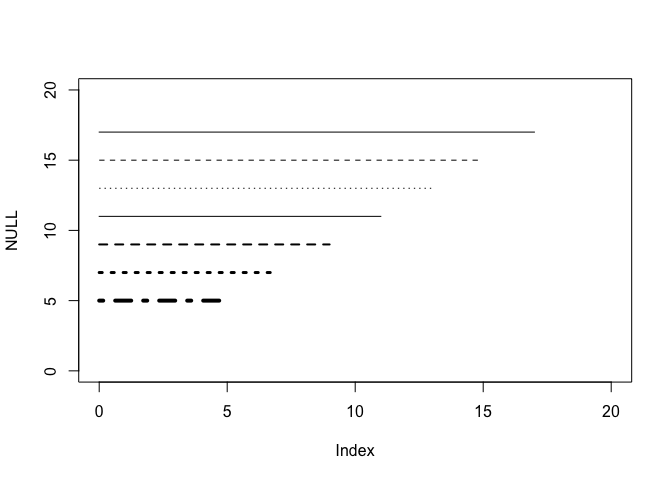
\includegraphics{part-2.-정리_files/figure-latex/unnamed-chunk-2-1.pdf}

\begin{Shaded}
\begin{Highlighting}[]
\FunctionTok{biplot}\NormalTok{(US\_prin,}\AttributeTok{scale =} \DecValTok{0}\NormalTok{)}
\end{Highlighting}
\end{Shaded}

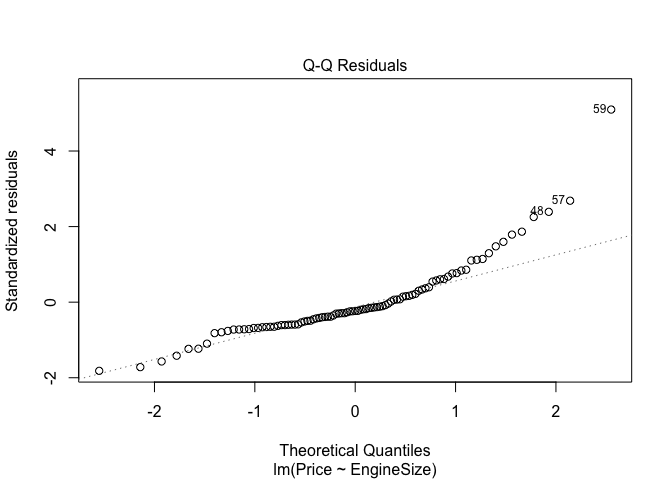
\includegraphics{part-2.-정리_files/figure-latex/unnamed-chunk-2-2.pdf}

\hypertarget{uxc694uxc778uxbd84uxc11d}{%
\paragraph{3. 요인분석}\label{uxc694uxc778uxbd84uxc11d}}

요인분석 : 변수들 간의 상관관계를 고려하여 서로 유사한 변수들을 묵어
새로운 잠재요인들을 추출

\begin{quote}
factanla(data, factors=n, rotation=`varimax',
scores=`regression',\ldots)

\begin{itemize}
\item
  factors : 요인의 개수 지정
\item
  rotation : 요인 회전방법(`varimax,'promax',`none')
\item
  scores : 요인점수 계산 방법(`regression',`Bartlett')
\end{itemize}
\end{quote}

\begin{Shaded}
\begin{Highlighting}[]
\FunctionTok{data}\NormalTok{(}\StringTok{"swiss"}\NormalTok{)}
\NormalTok{Min }\OtherTok{\textless{}{-}} \FunctionTok{apply}\NormalTok{(swiss,}\DecValTok{2}\NormalTok{,min)}
\NormalTok{Max }\OtherTok{\textless{}{-}} \FunctionTok{apply}\NormalTok{(swiss,}\DecValTok{2}\NormalTok{,max)}
\NormalTok{swiss\_fa }\OtherTok{\textless{}{-}} \FunctionTok{scale}\NormalTok{(swiss, }\AttributeTok{center=}\NormalTok{Min, }\AttributeTok{scale =}\NormalTok{ (Max}\SpecialCharTok{{-}}\NormalTok{Min))}

\CommentTok{\# i) 고유값을 통해 요인 개수 설정}
\NormalTok{swiss.prin }\OtherTok{\textless{}{-}} \FunctionTok{princomp}\NormalTok{(swiss, }\AttributeTok{cor =} \ConstantTok{TRUE}\NormalTok{)}
\NormalTok{swiss.prin}\SpecialCharTok{$}\NormalTok{sdev}\SpecialCharTok{\^{}}\DecValTok{2}
\end{Highlighting}
\end{Shaded}

\begin{verbatim}
##    Comp.1    Comp.2    Comp.3    Comp.4    Comp.5    Comp.6 
## 3.1997570 1.1883082 0.8476098 0.4389287 0.2045337 0.1208626
\end{verbatim}

\begin{Shaded}
\begin{Highlighting}[]
\CommentTok{\# =\textgreater{} 고유값이 1 이상인 개수를 요인 개수로 설정}

\CommentTok{\# ii) screeplot을 통해 요인 개수 설정}
\FunctionTok{plot}\NormalTok{(swiss.prin,}\AttributeTok{type=}\StringTok{\textquotesingle{}l\textquotesingle{}}\NormalTok{)}
\end{Highlighting}
\end{Shaded}

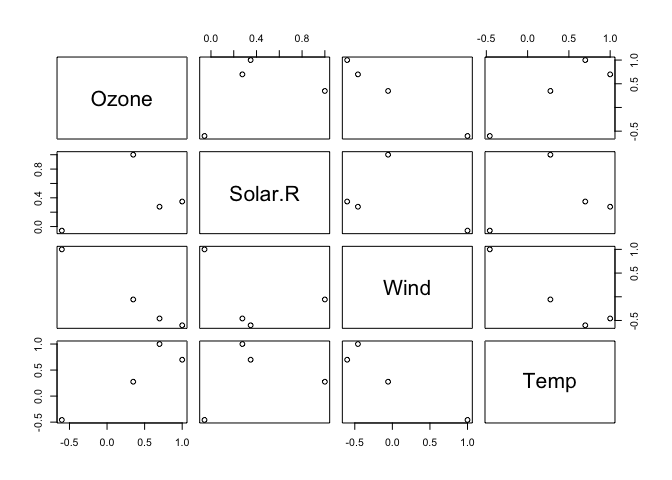
\includegraphics{part-2.-정리_files/figure-latex/unnamed-chunk-3-1.pdf}

\begin{Shaded}
\begin{Highlighting}[]
\CommentTok{\# =\textgreater{} 기울기가 완만해지는 점 전까지를 요인 개수로 설정}

\CommentTok{\# iii) cor(df)를 통해 직접 요인 개수 설정}
\FunctionTok{cor}\NormalTok{(swiss)}
\end{Highlighting}
\end{Shaded}

\begin{verbatim}
##                   Fertility Agriculture Examination   Education   Catholic
## Fertility         1.0000000  0.35307918  -0.6458827 -0.66378886  0.4636847
## Agriculture       0.3530792  1.00000000  -0.6865422 -0.63952252  0.4010951
## Examination      -0.6458827 -0.68654221   1.0000000  0.69841530 -0.5727418
## Education        -0.6637889 -0.63952252   0.6984153  1.00000000 -0.1538589
## Catholic          0.4636847  0.40109505  -0.5727418 -0.15385892  1.0000000
## Infant.Mortality  0.4165560 -0.06085861  -0.1140216 -0.09932185  0.1754959
##                  Infant.Mortality
## Fertility              0.41655603
## Agriculture           -0.06085861
## Examination           -0.11402160
## Education             -0.09932185
## Catholic               0.17549591
## Infant.Mortality       1.00000000
\end{verbatim}

\begin{Shaded}
\begin{Highlighting}[]
\CommentTok{\# =\textgreater{} 상관계수 값이 높은 그룹의 개수를 요인 개수로 설정}

\FunctionTok{factanal}\NormalTok{(swiss\_fa, }\AttributeTok{factors=}\DecValTok{2}\NormalTok{)}
\end{Highlighting}
\end{Shaded}

\begin{verbatim}
## 
## Call:
## factanal(x = swiss_fa, factors = 2)
## 
## Uniquenesses:
##        Fertility      Agriculture      Examination        Education 
##            0.420            0.492            0.270            0.005 
##         Catholic Infant.Mortality 
##            0.061            0.960 
## 
## Loadings:
##                  Factor1 Factor2
## Fertility        -0.652   0.393 
## Agriculture      -0.631   0.333 
## Examination       0.685  -0.510 
## Education         0.997         
## Catholic         -0.124   0.961 
## Infant.Mortality          0.175 
## 
##                Factor1 Factor2
## SS loadings      2.311   1.481
## Proportion Var   0.385   0.247
## Cumulative Var   0.385   0.632
## 
## Test of the hypothesis that 2 factors are sufficient.
## The chi square statistic is 20.99 on 4 degrees of freedom.
## The p-value is 0.000318
\end{verbatim}

\begin{Shaded}
\begin{Highlighting}[]
\CommentTok{\# =\textgreater{} Cumulative Var : 전체 데이터 분산의 \%를 설명}
\CommentTok{\# =\textgreater{} p{-}value : 기각=요인 분석 개수 적절X}
\end{Highlighting}
\end{Shaded}

\hypertarget{uxd45cuxc900uxd654uxc640-uxc815uxaddcuxd654}{%
\paragraph{4. 표준화와
정규화}\label{uxd45cuxc900uxd654uxc640-uxc815uxaddcuxd654}}

\begin{itemize}
\tightlist
\item
  표준화
\end{itemize}

\begin{quote}
scale(data,center,scale)
\end{quote}

\begin{itemize}
\tightlist
\item
  정규화
\end{itemize}

\begin{quote}
scale(data, center=Min, scale=Max-Min)
\end{quote}

\begin{Shaded}
\begin{Highlighting}[]
\FunctionTok{data}\NormalTok{(iris)}
\NormalTok{Min }\OtherTok{\textless{}{-}} \FunctionTok{apply}\NormalTok{(iris[}\DecValTok{1}\SpecialCharTok{:}\DecValTok{4}\NormalTok{],}\DecValTok{2}\NormalTok{,min)}
\NormalTok{Max }\OtherTok{\textless{}{-}} \FunctionTok{apply}\NormalTok{(iris[}\DecValTok{1}\SpecialCharTok{:}\DecValTok{4}\NormalTok{],}\DecValTok{2}\NormalTok{,max)}

\CommentTok{\# 표준화}
\FunctionTok{head}\NormalTok{(}\FunctionTok{scale}\NormalTok{(iris[}\DecValTok{1}\SpecialCharTok{:}\DecValTok{4}\NormalTok{]))}
\end{Highlighting}
\end{Shaded}

\begin{verbatim}
##      Sepal.Length Sepal.Width Petal.Length Petal.Width
## [1,]   -0.8976739  1.01560199    -1.335752   -1.311052
## [2,]   -1.1392005 -0.13153881    -1.335752   -1.311052
## [3,]   -1.3807271  0.32731751    -1.392399   -1.311052
## [4,]   -1.5014904  0.09788935    -1.279104   -1.311052
## [5,]   -1.0184372  1.24503015    -1.335752   -1.311052
## [6,]   -0.5353840  1.93331463    -1.165809   -1.048667
\end{verbatim}

\begin{Shaded}
\begin{Highlighting}[]
\CommentTok{\# 정규화}
\FunctionTok{head}\NormalTok{(}\FunctionTok{scale}\NormalTok{(iris[}\DecValTok{1}\SpecialCharTok{:}\DecValTok{4}\NormalTok{],}\AttributeTok{center=}\NormalTok{Min,}\AttributeTok{scale=}\NormalTok{Max}\SpecialCharTok{{-}}\NormalTok{Min))}
\end{Highlighting}
\end{Shaded}

\begin{verbatim}
##      Sepal.Length Sepal.Width Petal.Length Petal.Width
## [1,]   0.22222222   0.6250000   0.06779661  0.04166667
## [2,]   0.16666667   0.4166667   0.06779661  0.04166667
## [3,]   0.11111111   0.5000000   0.05084746  0.04166667
## [4,]   0.08333333   0.4583333   0.08474576  0.04166667
## [5,]   0.19444444   0.6666667   0.06779661  0.04166667
## [6,]   0.30555556   0.7916667   0.11864407  0.12500000
\end{verbatim}

\hypertarget{uxb370uxc774uxd130-uxacb0uxd569-uxbc0f-uxc694uxc57d}{%
\subsubsection{3. 데이터 결합 및
요약}\label{uxb370uxc774uxd130-uxacb0uxd569-uxbc0f-uxc694uxc57d}}

\hypertarget{uxacb0uxd569}{%
\paragraph{1. 결합}\label{uxacb0uxd569}}

\begin{quote}
rbind()
\end{quote}

\begin{quote}
cbind()
\end{quote}

\begin{quote}
merge()
\end{quote}

\hypertarget{uxc694uxc57d}{%
\paragraph{2. 요약}\label{uxc694uxc57d}}

\begin{quote}
aggregate()
\end{quote}

\begin{quote}
table()
\end{quote}

\begin{quote}
prop.table()
\end{quote}

\begin{quote}
subset()
\end{quote}

\hypertarget{apply}{%
\paragraph{3. apply}\label{apply}}

\begin{quote}
apply()
\end{quote}

\begin{quote}
lapply()
\end{quote}

\begin{quote}
sapply()
\end{quote}

\begin{quote}
vapply()
\end{quote}

\begin{quote}
mapply()
\end{quote}

\begin{quote}
tapply()
\end{quote}

\hypertarget{uxd328uxd0a4uxc9c0-uxc774uxc6a9}{%
\subsubsection{4. 패키지 이용}\label{uxd328uxd0a4uxc9c0-uxc774uxc6a9}}

\hypertarget{reshape2}{%
\paragraph{1. reshape2}\label{reshape2}}

\begin{quote}
\textbf{reshape2 패키지}

melt(df, id.vars, measure.vars) : 열을 행으로

\begin{itemize}
\item
  id.vars : 기준이 되는 식별자 칼럼들
\item
  measure.vars : 측정치 칼럼들
\end{itemize}
\end{quote}

\begin{quote}
\textbf{reshape2 패키지}

dcast(df, formula, fun.aggregate) : 행을 열로

\begin{itemize}
\item
  formula : id변수 \textasciitilde{} variable변수
\item
  fun.aggregate : id변수를 기준으로 여러 행이 존재할 경우 해당 행들에
  적용할 집합 함수
\end{itemize}
\end{quote}

\begin{Shaded}
\begin{Highlighting}[]
\FunctionTok{library}\NormalTok{(reshape2)}
\FunctionTok{data}\NormalTok{(}\StringTok{"airquality"}\NormalTok{)}
\NormalTok{dt }\OtherTok{\textless{}{-}}\NormalTok{ airquality}

\CommentTok{\# melt()}
\NormalTok{dt\_melt }\OtherTok{\textless{}{-}} \FunctionTok{melt}\NormalTok{(dt, }\AttributeTok{id.vars =} \FunctionTok{c}\NormalTok{(}\StringTok{\textquotesingle{}Month\textquotesingle{}}\NormalTok{,}\StringTok{\textquotesingle{}Day\textquotesingle{}}\NormalTok{), }\AttributeTok{na.rm =}\NormalTok{ T)}
\FunctionTok{head}\NormalTok{(dt\_melt)}
\end{Highlighting}
\end{Shaded}

\begin{verbatim}
##   Month Day variable value
## 1     5   1    Ozone    41
## 2     5   2    Ozone    36
## 3     5   3    Ozone    12
## 4     5   4    Ozone    18
## 6     5   6    Ozone    28
## 7     5   7    Ozone    23
\end{verbatim}

\begin{Shaded}
\begin{Highlighting}[]
\CommentTok{\# dcast()}
\FunctionTok{head}\NormalTok{(}\FunctionTok{dcast}\NormalTok{(dt\_melt, Month}\SpecialCharTok{+}\NormalTok{Day}\SpecialCharTok{\textasciitilde{}}\NormalTok{...))}
\end{Highlighting}
\end{Shaded}

\begin{verbatim}
##   Month Day Ozone Solar.R Wind Temp
## 1     5   1    41     190  7.4   67
## 2     5   2    36     118  8.0   72
## 3     5   3    12     149 12.6   74
## 4     5   4    18     313 11.5   62
## 5     5   5    NA      NA 14.3   56
## 6     5   6    28      NA 14.9   66
\end{verbatim}

\hypertarget{uxacb0uxce21uxce58}{%
\subsubsection{5. 결측치}\label{uxacb0uxce21uxce58}}

\hypertarget{uxacb0uxce21uxce58-1}{%
\paragraph{1. 결측치}\label{uxacb0uxce21uxce58-1}}

\begin{itemize}
\tightlist
\item
  결측치 확인
\end{itemize}

\begin{quote}
is.na()
\end{quote}

\begin{quote}
complete.cases()
\end{quote}

\begin{itemize}
\tightlist
\item
  결측치 처리
\end{itemize}

\begin{enumerate}
\def\labelenumi{\arabic{enumi}.}
\item
  결측치 제거
\item
  중앙값/평균값/최빈값/상수값 대치

  \begin{quote}
  \textbf{DMwR 패키지 (깃허브를 통해)}

  centralImputation(data) : 중앙값

  centralValue(data) : 중앙값 / 최빈값
  \end{quote}
\item
  K-NN

  \begin{quote}
  \textbf{DMwR 패키지 (깃허브를 통해)}

  knnImputation(data, k)
  \end{quote}
\item
  MICE(Multivariate Imputation by Chained Equation)
\item
  딥러닝을 활용한 Imputation
\end{enumerate}

※ 가이드라인\\
10\% 미만 : 삭제 or 대치\\
10\% \textasciitilde{} 50\% : regression or model based imputation\\
50\% 이상 : 해당 변수 자체 제거

\hypertarget{uxc774uxc0c1uxce58}{%
\paragraph{2. 이상치}\label{uxc774uxc0c1uxce58}}

\begin{quote}
quantile()
\end{quote}

\begin{quote}
fivenum()
\end{quote}

\begin{quote}
summary()
\end{quote}

\begin{quote}
boxplot()
\end{quote}

\hypertarget{uxb0a0uxc9dc-uxb370uxc774uxd130}{%
\subsubsection{6. 날짜 데이터}\label{uxb0a0uxc9dc-uxb370uxc774uxd130}}

\begin{quote}
Sys.Date() : 현재 날짜
\end{quote}

\begin{quote}
Sys.time() : 현재 날짜와 시간
\end{quote}

\begin{quote}
as.Date()
\end{quote}

\begin{quote}
as.POSIXct()
\end{quote}

\begin{quote}
as.POSIXlt()
\end{quote}

\hypertarget{uxd074uxb798uxc2a4uxbd88uxade0uxd615}{%
\subsubsection{7.
클래스불균형}\label{uxd074uxb798uxc2a4uxbd88uxade0uxd615}}

\begin{itemize}
\tightlist
\item
  업 샘플링 / 다운 샘플링
\end{itemize}

\begin{quote}
\textbf{caret 패키지}

upSample(x, y)

downSample(x, y)
\end{quote}

\begin{itemize}
\tightlist
\item
  SMOTE
\end{itemize}

\begin{quote}
\textbf{DMwR 패키지 (깃허브를 통해)}

SMOTE(form, data, perc.over, k, perc.under)
\end{quote}

\end{document}
